\section{Measuring}

\begin{frame}
\frametitle{Time measurement equipment: hardware}
\begin{itemize}
\item The best equipment is an oscilloscope, if you can afford one
\item Allows to time the "Power on" event (connected to a power rail),
      or any event (connected to a GPIO pin, for example), all this
      in a very accurate way.
\item Easy to write to a GPIO at all the stages of system booting
      (we will explain how to do it)
\item Some oscilloscopes are getting affordable. Example: Bitscope
      Pocket Analyzer (245 AUD, supported on Linux, \url{https://www.bitscope.com/product/BS10/})
\end{itemize}
\begin{center}
    % From http://openclipart.org/detail/28033/oscilloscope-by-mothinator
    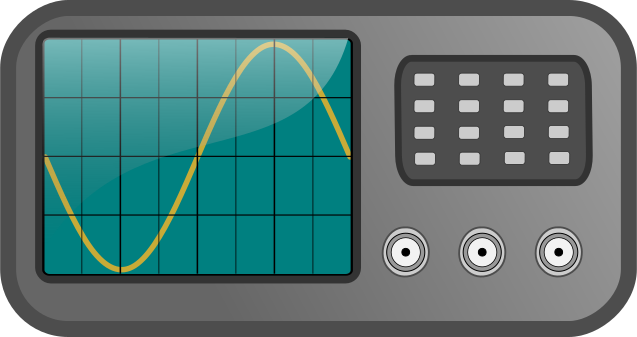
\includegraphics[width=0.35\textwidth]{slides/boot-time-measuring/mothinator_Oscilloscope.pdf}
\end{center}
\end{frame}

\begin{frame}
\frametitle{Measuring with hardware: using an Arduino}
\begin{columns}
\column{0.85\textwidth}
  \url{https://arduino.cc}
  \begin{itemize}
  \item If you don't have an oscilloscope, an Arduino (or any general
        purpose MCU or MPU board) is a great solution too.
  \item The main strength of Arduino is its great ease of use and
        programming, plus all the hardware support libraries that are available.
  \item You can easily connect board pins to the Arduino analog pins, and
        watch their voltage.
  \item In our labs, we will use Arduino Nano boards for measuring the
        whole boot time.
  \item Arduino boards are Open Source Hardware. This project is
      definitely worth supporting!
  \end{itemize}
\column{0.15\textwidth}
  \begin{center}
  \tiny
  % From https://commons.wikimedia.org/wiki/File:Arduino_Logo.svg
  \includegraphics[width=0.5\textwidth]{slides/boot-time-measuring/arduino-logo.pdf}\\
  \vspace{1cm}
  Arduino Nano\\
  % From https://commons.wikimedia.org/wiki/File:Arduino_nano_isometr.jpg
  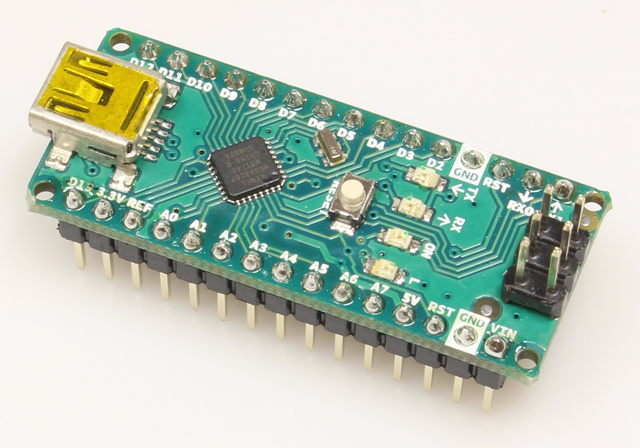
\includegraphics[width=\textwidth]{slides/boot-time-measuring/arduino-nano.jpg}\\
  Image credits: \url{https://frama.link/wdhQENrp} (Wikimedia Commons)\\
  \vspace{1cm}
  
\includegraphics[width=0.5\textwidth]{slides/beagleboneblack-board/open-source-hardware-logo.pdf}
  \end{center}
\end{columns}
\end{frame}

\begin{frame}
\frametitle{Time measurement equipment: serial port}
\begin{columns}
\column{0.75\textwidth}
\begin{itemize}
\item Useful when you don't have monitoring hardware, or don't want to make
      take any risk connecting wires to the hardware.
\item Usually relies on software which times messages received from the board's
      serial port (serial port absolutely required). Such software
      runs on a PC connected to the serial port.
\item On the board, requires a real serial port (directly connected to the CPU),
      immediately usable from the earliest parts of the boot process.
\item Limitation: won't be able to time the "Power on" event in
      an accurate way. But acceptable as you can assume that
      the time to run the first stage bootloader is constant.
\end{itemize}
\column{0.25\textwidth}
% From http://openclipart.org/detail/173570/serial-db9-female-by-deusinvictus-173570

\includegraphics[width=\textwidth]{slides/boot-time-measuring/serial_db9_female.pdf}
\end{columns}
\end{frame}

\begin{frame}
\frametitle{Time measurement equipment: USB to serial}
\begin{columns}
    \column{0.65\textwidth}
	\begin{itemize}
	\item Serial ports over USB {\bf device} are fine if there's an on-board
	      serial-to-USB chip directly connected to the CPU serial port (very frequent).
	\item Attaching a USB-to-serial dongle to a USB {\bf host} port on
	      the device won't do: USB is available much later and messages
	      go through more complex software stacks (loss of time accuracy).
	\item All development boards have a standard or USB serial port.
	\end{itemize}
    \column{0.35\textwidth}
	% From http://openclipart.org/detail/135721/usb-cable-by-gsagri04
	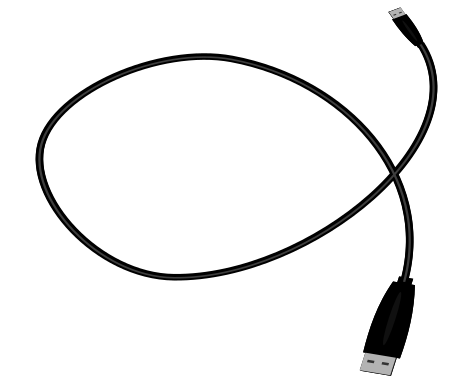
\includegraphics[width=\textwidth]{slides/boot-time-measuring/GS_USB_Cable.pdf}
\end{columns}
\end{frame}

\begin{frame}
\frametitle{grabserial}
\begin{itemize}
\item From Tim Bird: \url{https://elinux.org/Grabserial}
\item A Python script to add timestamps to messages coming from a
	serial console.
\item Key advantage: starts counting very early (bootstrap and bootloader)
\item Another advantage: no overhead on the target, because run on the host machine.
\item Drawbacks: may not be precise enough. Can't measure power up time.
\end{itemize}
\end{frame}

\begin{frame}
\frametitle{Using grabserial}
\begin{center}
    \includegraphics[height=0.65\textheight]{slides/boot-time-measuring/using-grabserial.pdf}
\end{center}
{\small
{\bf Caution}: \code{grabserial} shows the arrival time of the
{\bf first character} of a line. This doesn't mean that the entire line
was received at that time.}
\end{frame}

\begin{frame}
\frametitle{grabserial tips}
\begin{itemize}
  \item You can interrupt \code{grabserial} manually (with
  \code{[Ctrl][c]}) when you have gone far enough.
  \item The \code{-m} and \code{-q} options actually expect a regular expression.
  A normal string may not match in the middle of a line.
  \item Example: you may have to replace \code{-m "Starting kernel"} by
  \code{-m ".*Starting Kernel.*"}. 
\end{itemize}
\end{frame}

\begin{frame}
\frametitle{Dedicated measuring resources}
Later, we will see specific resources for measuring time
\begin{itemize}
  \item \code{strace} for application tracing
  \item \code{bootchartd} for tracing the execution of system services
  \item \code{CONFIG_PRINTK_TIME} and \code{initcall_debug} for
        tracing kernel code and functions.
\end{itemize}
\end{frame}


\setuplabframe {Measuring time}
{
Measuring time with software
\begin{itemize}
\item Setting up \code{grabserial}
\item Modify the video player to log a notification
      after the first frame is processed.
\item Time the various components of boot time through messages
      written to the serial console.
\end{itemize}

Measuring time with hardware
\begin{itemize}
\item Setting up an Arduino system
\item Timing reset on Beagle Bone Black
\item Modifying the video player to toggle a GPIO
      after the first frame is processed.
\item Display the live total time through a 7-segment display
\end{itemize}
}
